\documentclass{SchoolBook}

\usepackage{enumitem}
\usepackage{multicol}
\usepackage{xcolor}
\usepackage{tikz}

\setlength{\parskip}{3pt}

\begin{document}
    \begin{day}{22/04/2021}
        \title{3}{Leia o texto a seguir e responda às questões.}
        \title{4}{Turma da Mônica: Laços}
        
        Filme da turminha é exemplo de adaptação e garantia de agrado aos fãs

        Quando foi anunciada a produção de um live-action da Turma da Mônica, foi difícil não ficar com um pé atrás. A hesitação é normal, já que qualquer adaptação de obra literária é arriscada, mas no caso da turminha que existe nos quadrinhos desde o fim dos anos 50, a questão era mais pessoal para o público brasileiro. [...]

        Laços tem um ritmo único que combina adaptação de HQs e filme infantil, sem perder timing de piadas e seguindo uma estrutura de aventura juvenil. [...]

        Enquanto todos os aspectos técnicos de Laços são dignos de menção, existe algo que fez do filme o que ele é, e que sem ele o projeto poderia ruir por completo: o elenco. [...] Daniel Rezende escolheu mostrar seus personagens sem flashbacks de origem, e tomou a liberdade de inserir certos elementos de Lições, a HQ seguinte, neste primeiro filme. [...]

        Por fim, Turma da Mônica: Laços marca o cinema nacional como uma obra exemplar de técnica, carisma, e adaptação de um dos nossos maiores patrimônios. É delicioso testemunhar o comprometimento da produção com o longa, o que faz com que cada fã do público se sinta representado de alguma forma pelo trabalho de Daniel Rezende. A sensação de que um fã qualificado tomou algo tão querido nas mãos é gratificante.

        \title{3}{ATIVIDADE}

        \begin{enumerate}
            \item[1.] Do que trata o texto?
            \response Sobre um filme adaptado dos quadrinhos.
            %O texo se trata sobre o \emph{live-action} Turma da Mônica: Laços.

            \item[2.] Que tipo de informação apresenta?
            \response Informações técnicas e analíticas.
            %Quando foi anunciado, criação e um pouco da obra original, como foi feita, elenco, opinião do escritor.

            \item[3.] É um texto descritivo ou opinativo? Justifique.
            \response Ambos. Descrevem alguns aspectos sobre a obra, acrecidos da opinião do autor do texto.
            %Um pouco de ambos, no início o autor descreve um pouco da obra, e o final dá opinião sobre a obra.

            \item[4.] Há pontos positivos e/ou negativos? Encontre-os.
            \response Somente pontos positivos. Aspectos técnicos e escolhas da direção.
        \end{enumerate}

        \title{3}{Importante lembrar\dots}

        A resenha é um texto sucinto, cuja principal característica é tecer, de maneira breve, uma crítica sobre determinado assunto.

        A resenha ideal é composta não apenas pela crítica direta, mas também por momentos de descrição, e esses dois elementos devem estar em perfeito equilíbrio em seu texto.
        
        \vspace{3pt}
        A resenha difere-se de um resumo porquê?
        \vspace{3pt}

        \begin{enumerate}[nosep]
            \item[a)] apresenta informações técnicas.
            \item[b)] apresenta informações polêmicas.
        \bf \item[c)] apresenta análises e opiniões. \normalfont
            \item[d)] apresenta gráficos e tabelas.
        \end{enumerate}

        \title{3}{ATIVIDADE}
        Indique, abaixo, o que é FATO e o que é OPINIÃO:
        \vspace{3pt}

        \begin{enumerate}[nosep]
        \bf \item[1.] "Mas no caso da turminha que existe nos quadrinhos desde o fim dos anos 50." \normalfont
        \bf \item[2.] "A inspiração dos Cafaggi para a \emph{graphic novel} veio de filmes infanto-juvenis dos anos 80." \normalfont
            \item[3.] "Eu, pelo menos, nunca tinha visto aquela estratégia infalível contra a Mônica."
            \item[4.] "Todos os aspetos técnicos de Laços são dignos de menção."
        \end{enumerate}
    \end{day}

    \begin{day}{23/04/2021}
        \title{3}{Orações Subordinadas Adverbiais}
        
        Exercem a função do advérbio e funcionam como adjunto adverbial, sendo classificadas em:

        \begin{multicols}{3}
            \begin{itemize}[nosep]
                \item Causais;
                \item Comparativas;
                \item Concessivas;
                \item Condicionais;
                \item Conformativas;
                \item Consecutivas;
                \item Finais;
                \item Temporais;
                \item Proporcionais.
            \end{itemize}
        \end{multicols}

        \title{3}{O que é Oração Subordinada Adverbial}

        Exemplo: ela partiu \underline{quando anoitecia}.
        \vspace{3pt}

        \begin{enumerate}[nosep]
            \item[a)] é subordinada porque completa a principal (\emph{ela partiu}).
            \item[b)] é adverbial porque apresenta uma circunstância de tempo (quando anoitecia, ao anoitecer)
        \end{enumerate}

        \vspace{8pt}
        Oração Subordinada Adverbial é, portanto, aquela que completa o sentido da principal

        \title{3}{ATIVIDADE}

        Localize as orações subordinadas adverbiais e classifique-as como Condicional, Conformativa ou Consecutiva:
        \vspace{3pt}

        \begin{enumerate}[nosep]
                \item[1.] \makebox[2.6cm][c]{(\textbf{Conformativa})} A história segue um ritmo \underline{como o conhecido nos desenhos da turminha}.
                \item[2.] \makebox[2.6cm][c]{(\textbf{Conformativa})} Escolheram o elenco \underline{segundo sua proximidade com os personagens originais}.
                \item[3.] \makebox[2.6cm][c]{(\textbf{Condicional})}  Tudo poderia ruir \underline{se não fosse o elenco afinado}.
                \item[4.] \makebox[2.6cm][c]{(\textbf{Consecutiva})}  A produção adaptou os quadrinhos \underline{sem que o público estranhasse}.
        \end{enumerate}

        \title{3}{Resenha de Filmes\\(e de outras obras também)}

        A função de uma resenha é ir um pouco mais a fundo na obra analisada, trazendo críticas sobre determinados pontos da produção, além de outras referências.

    \end{day}
    
    \begin{day}{29/04/2021}
        Mário de Andrade estreou em 1917 com "Há uma gota de sangue em cada poema". Só em 1922 com "Paulicéia Desvairada", se torna modernista.
        
        "Paulicéia Desvairada", "Macunaíma", "Amar: Verbo Intransitivo" e "Lira Paulistana"
        
        Nas duas primeiras décadas do sec XX ocorreram várias transformações sociais: Urbanização, Imigração e Deslocamento dos Escravos.
        
        Agitações sociais, movimentos grevistas, visão crítica dos escritores.
    \end{day}
    
    \begin{day}{10/06/2021}
        \title{3}{Editorial}
        
        Estrutura: Introdução, desenvolvimento e conclusão.
        
        \begin{itemize}[nosep]
            \item Uma tese; uma ideia a ser defendida por um conjunto de editores responsáveis pelas publicações;
            \item Escrito na terceira pessoa do singular, onde o autor é implícito e impessoal;
            \item Assinado por uma instituição, não por uma pessoa;
            \item Apresenta dados que sustentam o posicionamento, bem como estatísticas e alusões históricas;
            \vspace{6pt}
            \item Não possui público-alvo; o público-alvo buscará a publicação, uma vez para verificar se assemelha ou não aos seus ideais;
            \item O texto é informativo, mas também argumentativo e enfático;
            \item Apresenta argumentos que defendem a posição e podem conter refutações às opiniões contrárias.
        \end{itemize}
    \end{day}
    
    \begin{day}{18/06/2021}
        \title 3 {O que é artigo de opinião?}
        
        Texto dissertativo, em que o autor expõe seu posicionamento diante de algum tema atual e interesse de muitas pessoas.
        
        Geralmente escrito por espeialistas e profissionais com muita experiência no assunto.
        
        \vspace{16pt}
        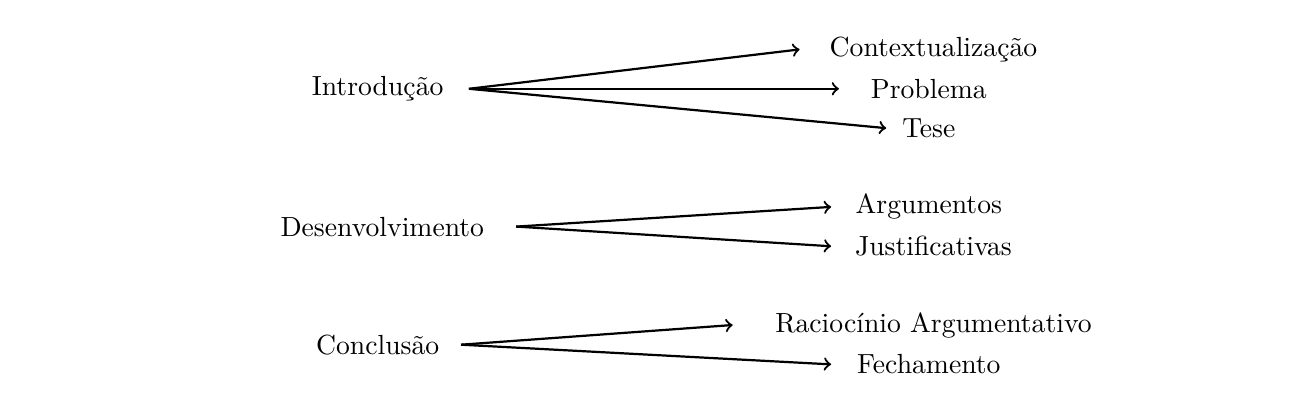
\begin{tikzpicture}\setmainfont{Latin Modern Roman}
            % Change from white to gray to enable grid
            \draw [very thin, white,step=1] (-8,0) grid (8,-4);
           %\filldraw [fill=black] (0,0) circle [radius=1.5pt];
            
            \coordinate (textA) at (-3.5,-0.5);
            \coordinate (textB) at (-3.5,-2.25);
            \coordinate (textC) at (-3.5,-3.75);
            
            \coordinate (A) at (-2.4,-0.5);
            \coordinate (B) at (-1.8,-2.25);
            \coordinate (C) at (-2.5,-3.75);
            
            \node [align=center] at (textA) {Introdução     };
            \node [align=center] at (textB) {Desenvolvimento};
            \node [align=center] at (textC) {Conclusão      };
            
            \coordinate (textAa) at (3.5,0);
            \coordinate (textAb) at (3.5,-0.5);
            \coordinate (textAc) at (3.5,-1);
            
            \coordinate (Aa) at (1.8,0);
            \coordinate (Ab) at (2.3,-0.5);
            \coordinate (Ac) at (2.9,-1);
            
            \node [align=center] at (textAa) {Contextualização};
            \node [align=center] at (textAb) {Problema        };
            \node [align=center] at (textAc) {Tese            };
            
            \coordinate (textBa) at (3.5,-2);
            \coordinate (textBb) at (3.5,-2.5);
            
            \coordinate (Ba) at (2.2,-2);
            \coordinate (Bb) at (2.2,-2.5);
            
            \node [align=center] at (textBa) {Argumentos    };
            \node [align=center] at (textBb) {Justificativas};
            
            \coordinate (textCa) at (3.5,-3.5);
            \coordinate (textCb) at (3.5,-4);
            
            \coordinate (Ca) at (0.95,-3.5);
            \coordinate (Cb) at (2.2,-4);
            
            \node [align=center] at (textCa) {Raciocínio Argumentativo};
            \node [align=center] at (textCb) {Fechamento              };
            
            \draw [->,thick] (A) -- (Aa);
            \draw [->,thick] (A) -- (Ab);
            \draw [->,thick] (A) -- (Ac);
            
            \draw [->,thick] (B) -- (Ba);
            \draw [->,thick] (B) -- (Bb);
            
            \draw [->,thick] (C) -- (Ca);
            \draw [->,thick] (C) -- (Cb);
        \end{tikzpicture}
        \title 4 {Título}
        
        É a parte mais "vendedora" do texto. Deve dar água na boca, mas não pode entregar o outro! Dica: seja simples, brinque, use clichês. É importante usar verbos para dar comandos de ação.
        
        Lembre-se: a afirmação deve ser intrigante, mas absolutamente comprovável.
        
        \title 4 {Introdução}
        
        Inicie sua tese apresentando ao leitor a problemática a ser discutiva. Dica: sempre que possível, contextualize om o cenário global ou algum acontecimento do dia a dia do seu leitor-alvo.
        
        Mostre que você não está sozinho: inclua afirmações de outros pensadores ou cite estatísticas, estudos científicos, reportagens de importantes veículos de comunicação.
        
        Use no máximo dois parágrafos (se conseguir num só, perfeito!).
        
        \title 4 {Desenvolvimento}
        
        Apresente seus argumentos.
        
        Justifique o por quê das suas afirmações (inclua o leitor; prenda-o em seus argumentos, fazendo com que ele se sinta representado por suas palavras).
        
        Neste trecho, seu leitor já começa a formatar suas próprias conclusões e você o está preparando para o \emph{gran finale}.
        
        \title 4 {Conclusão}
        
        \textbf{Raciocínio argumentativo}: agora é a hora de você mostrar ao leitor suas resoluções sobre o que foi apresentado e discutido.
        
        Proponha soluções, mostre um caso do qual você participou, indique o que foi feito; \underline{opine}.
        
        Você também pode deixar no ar um dúvida ou obrança. Se a intridução e o desenvolvimento foram perfeitos, seus leitores irão perdoá-lo.
        
        \textbf{Gran finale}: amarre o fim do seu texto com suas primeiras frases ou, então, jusifique o título com uma frase ao estilo "pulo do gato".
        
        \title 4 {Dicas}
        
        \begin{itemize}
            \item Só escreva sobre o que você domina e se tiver, realmente, algo a acrescentar sobre o assunto.
            \item Jogue todas as suas ideias no papel e só depois preocupe-se com a estrutura. Refaça quantas vezes precisar.
            \item Estimule seu poder de síntese -- menos é sempre mais!
            \item Faça parágrafos com no máximo quatro linhas. Intercale frases longas com outras mais curtas.
            \item Escreva de forma simples, evitando termos técnicos. Assim você alcançará um número maior de leitures -- que chegarão até o fim da leitura.
            \item Se você tiver problemas com o uso dos "por quês", substitua por "pois". Isso vale para outros termos e regras gramaticais.
            \item Tenha uma gramática sempre por perto.
            \item Evite repetir termos ou palavras. Enriqueça seu estoque de sinônimos.
            \item Lembre-se: o processo de comunicação só estará completo se o receptor entender a mensagem. Não jogue sua sabedoria ao vento. Seja simples e despresentioso ao redigir.
            \item Submeta seu texto a segundos e terceiros antes de publicar. Invariavelmente, ficamos "cegos" diante de erros ínfimos.
        \end{itemize}
    \end{day}
    
    \begin{day}{24/06/2021}
        O artigo de opinião caracteriza-se por omentar, analisar e opinar sobre fatos relevantes para a sociedade, que estão em destaque na mídia.
        
        \title 3 Atividade
        
        Na sua opinião, as redes sociais são um vício ou uma necessidade? Levante pelo menos 3 argumentos para defender seu ponto de vista.
        
        Depende do uso.
        
        Até um certo ponto as redes sociais podem ajudar a trazer informação para a pessoa, ser apenas um passa-tempo ou algo para descontrair de vez em quando. Porém quando o uso fica exagerado começa a gerar vício para o usuário, deixando-o dependente do uso, fazendo-o parar ou nem fazer tarefas obrigatórias do dia a dia ou diminuindo sua saúde mental.
        
        \title 3 {Estrutura de todo texto opinativo-argumentativo}
        
        \textbf{Introdução}: exposição do assunto que será tratado no decorrer da leitura;
        \textbf{Desenvolvimento}: momento em que a argumentação do escritor será a principal ferramenta;
        \textbf{Conclusão}: finalização do texto com 
        
        Escreva sua opinião sobre o uso da tecnologia atual em um texto de até 15 minhas. Opine sobre a necessidade.
    \end{day}
\end{document}
